\subsubsection{Exploration of the hyperparameters of the neural network}

To obtain the optimal neural network, we need to tune a series of hyperparameters, namely the \textit{number of hidden layers}, the \textit{size of the hidden layers}, as well as the choice of \textit{activation function}. The results from the in-depth exploration of these are presented in Figs. \ref{fig:boxplots_activations}, \ref{fig:boxplots_size_of_layers} and \ref{fig:boxplots_number_of_hidden_layers} respectively. 
From the three-dimensional grid search, the best values were found to be three hidden layers with size 50, and tanh as activation function.
Each of the figures (\ref{fig:boxplots_activations}, \ref{fig:boxplots_size_of_layers}, \ref{fig:boxplots_number_of_hidden_layers}) are made by keeping two of the three abovementioned hyperparameters constant, while varying the third as described on each $x$-axis.
The values for the constant hyperparameters are those producing the best model in the 3D grid search, i.e. layer size 50, 3 hidden layers, and tanh as activation function in the hidden layers.
The MSE of the best neural network is $ 6.71 \times 10^{-6}$.\label{best_nn_mse}
For each configuration, we have trained 10 separate models, using different seeds.
Hence the results should be robust with respect to random initializations.

\begin{figure}[h!]
    \centering
    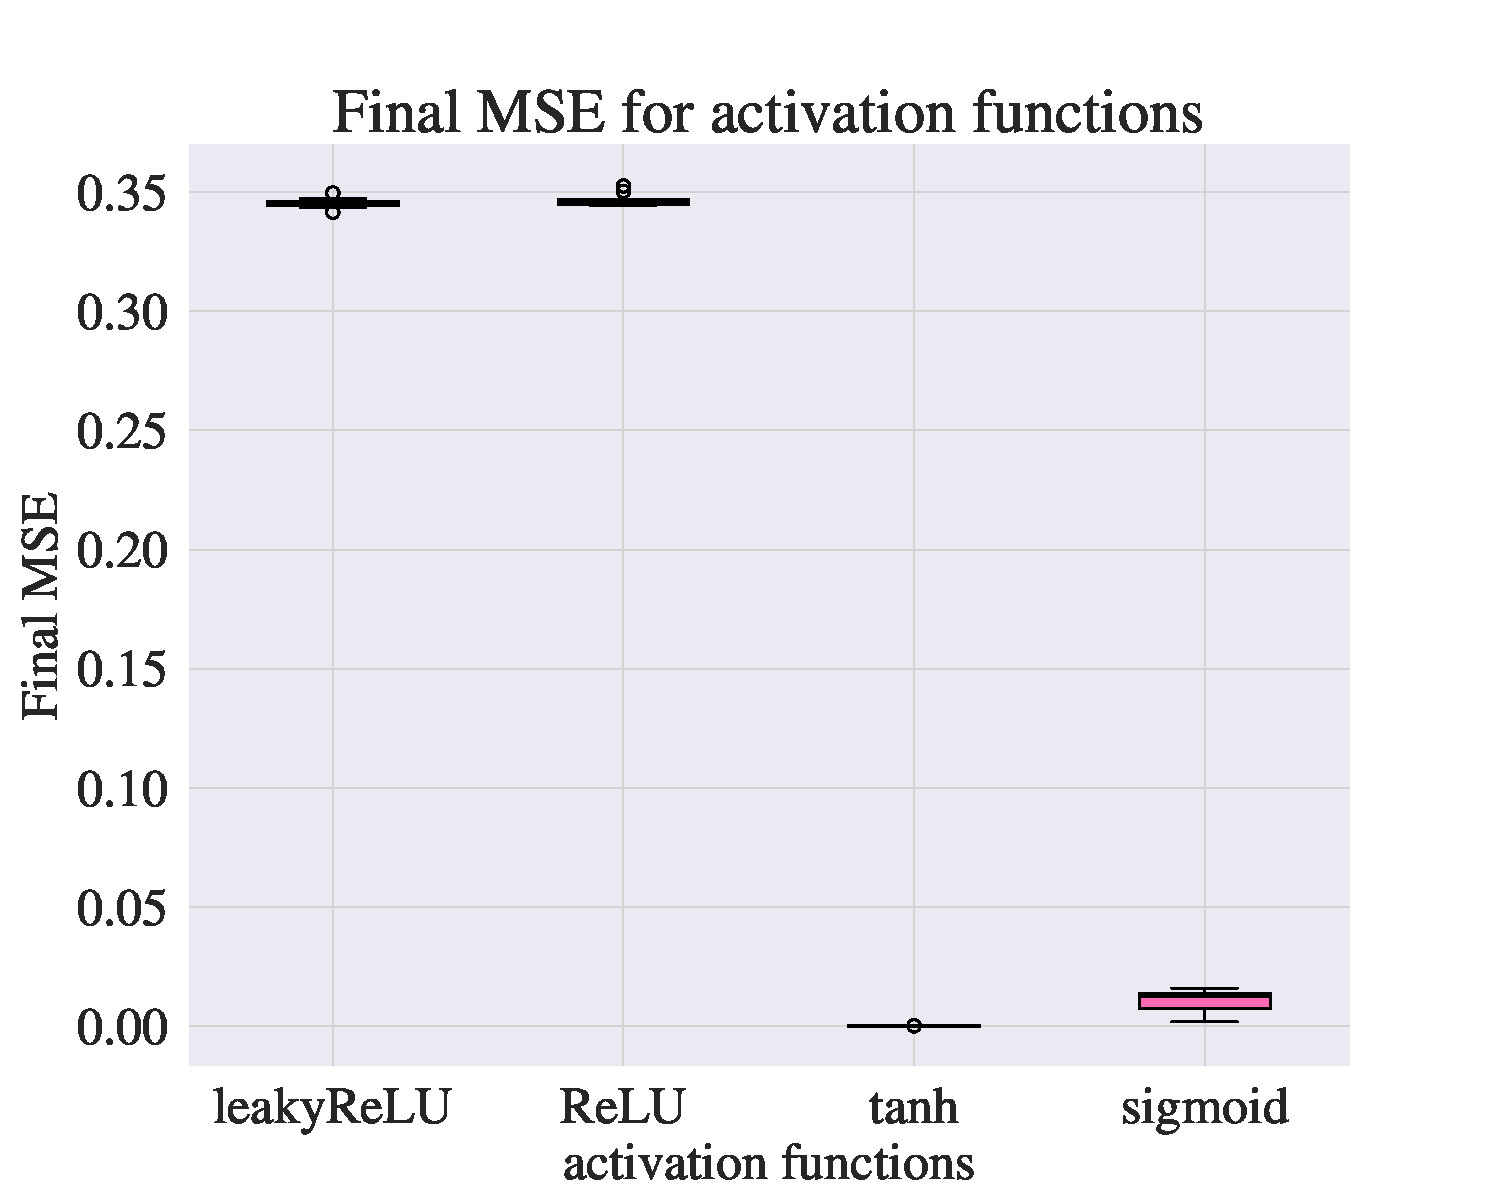
\includegraphics[width=1.0\linewidth]{project_3/plots/activation_search.pdf}
    \caption{Boxplots showcasing the final MSE value compared to the analytical solution for different activation functions. Each model is run 10 times.}
    \label{fig:boxplots_activations}
\end{figure}

%Mean MSE for activation = leakyReLU: 0.34531696140766144
% Mean MSE for activation = ReLU: 0.3466638922691345
% Mean MSE for activation = tanh: 1.579682736974064e-05
% Mean MSE for activation = sigmoid: 0.010715706355404109

As activation functions, sigmoid and tanh outperform ReLU and leakyReLU. 
The two former force the raw output from a node to a set range of values, $(0,1)$ and $(-1,1)$ respectively. 
The variants of ReLU, however, do not truncate the high positive values of the outputs from the nodes. 
Given the nature of the problem, it is highly intuitive that the ReLU-variants perform poorly. 
Furthermore, the analytical solution is known to have an output range [0,1]. 
Therefore, it is interesting to discuss why tanh does better than sigmoid, given that the latter yields output in the same range. 
However, this should not really matter as these activation functions are only used for the hidden layers.
That means their output range should not have a direct impact on the possible output range of the model.
We see no obvious reason why tanh should be performing better than sigmoid.
One of the problems with neural networks in general, is indeed the lack of interpretability of why some structures perform better than others.


\begin{figure}[h!]
    \centering
    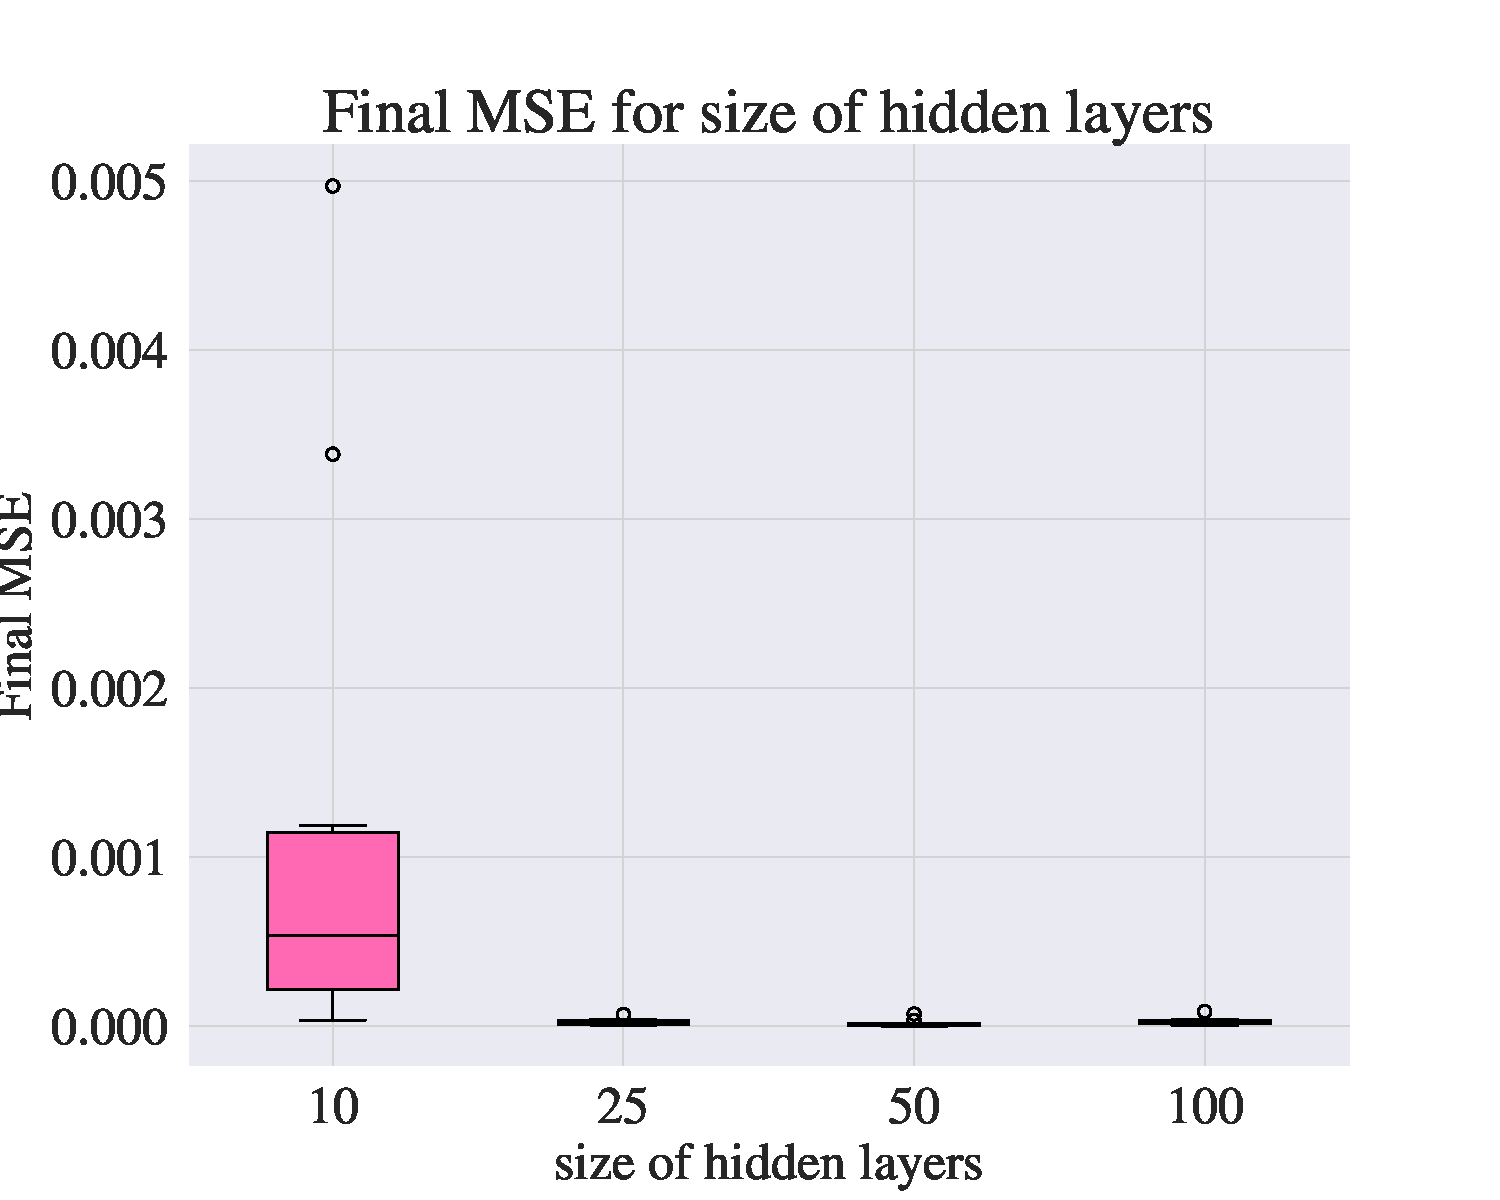
\includegraphics[width=1.0\linewidth]{project_3/plots/value_layers_search.pdf}
    \caption{Boxplots showcasing the final MSE value compared to the analytical solution for different sizes for the hidden layers. Each model is run 10 times. The y-axis is cut off to better visualize the content of the plot. Some outliers for hidden layers of size $10$ are consequently not displayed.}
    \label{fig:boxplots_size_of_layers}
\end{figure}

% Mean MSE for value_layers = 10: 0.0012251243981154403
% Mean MSE for value_layers = 25: 2.3295253322430652e-05
% Mean MSE for value_layers = 50: 1.579682736974064e-05
% Mean MSE for value_layers = 100: 3.0093467512415372e-05

The width of the neural network is decided by the size of the hidden layers.
In Fig. \ref{fig:boxplots_size_of_layers} one can see that a size of 10 is producing the poorest result, suggesting the NN does not capture the complexity of the problem with this width. 
The other widths are harder to distinguish by eye and we therefore present the mean MSE for each of them. 
The rest of this sub-section will by MSE refer to this mean MSE for the 10 models of each structure considered.
For hidden layers of size $25$ the MSE is $2.32 \times 10^{-5}$, for $50$ the MSE is $1.57 \times 10^{-5}$ and lastly, for 100 it is $3.00 \times 10^{-5}$.
There is an increase in performance as the width of the NN increases up to $50$. 
As the models do not seem to improve at all past this point, we conclude that $50$ nodes per hidden layer is optimal.
We in general favor smaller, simpler networks when the performance is similar.

\begin{figure}[h!]
    \centering
    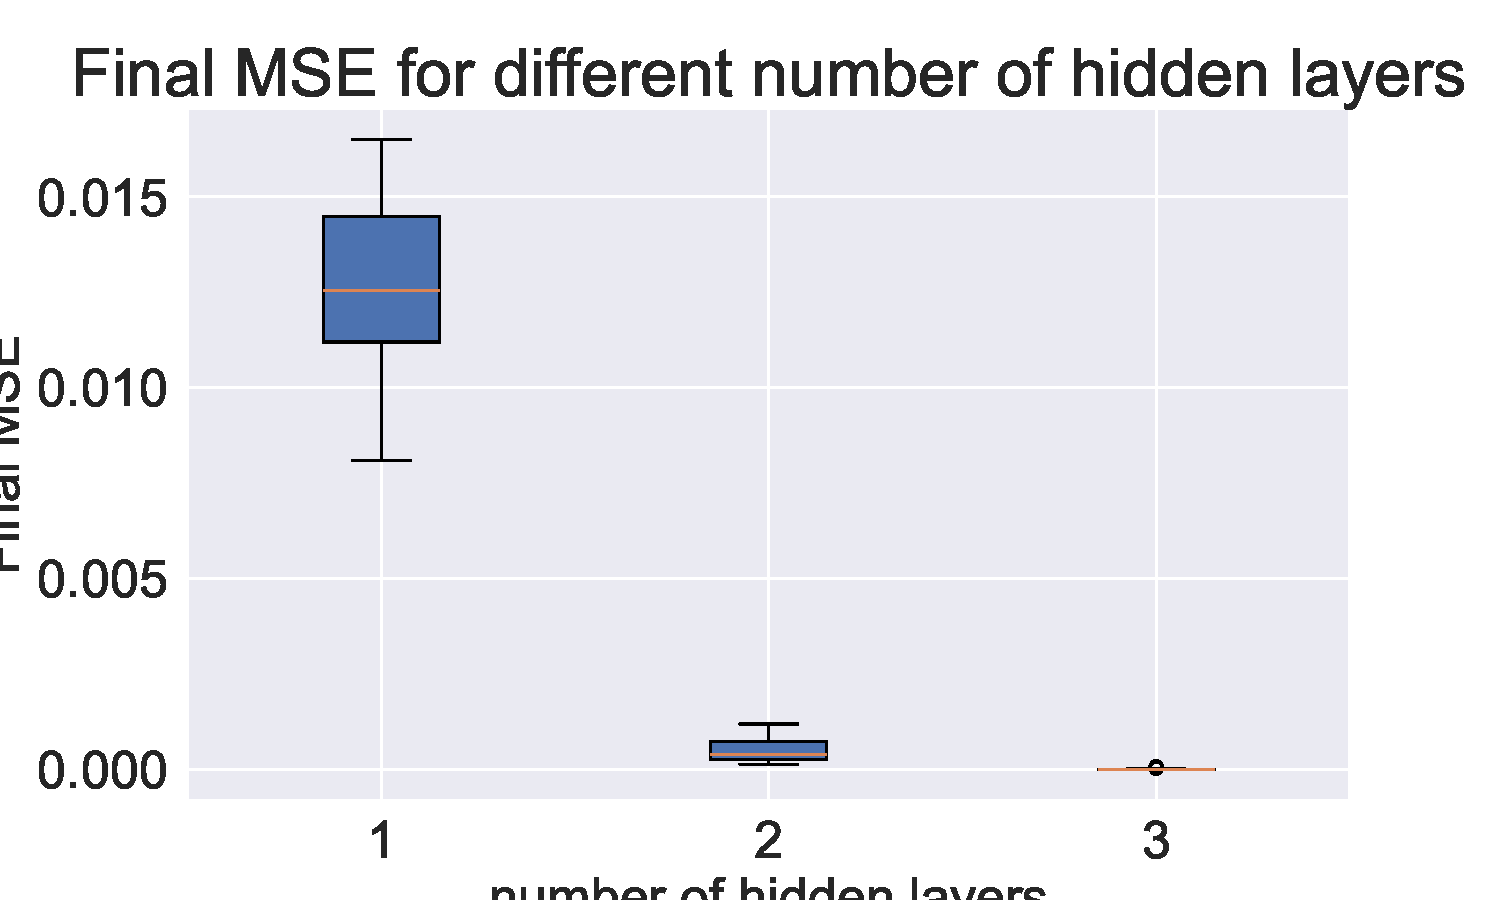
\includegraphics[width=1.0\linewidth]{project_3/plots/n_layers_search.pdf}
    \caption{Boxplots showcasing the final MSE value compared to the analytical solution for different numbers of hidden layers. Each model is run 10 times.}
    \label{fig:boxplots_number_of_hidden_layers}
\end{figure}

% Mean MSE for n_layers = 1: 0.012613625824451446
% Mean MSE for n_layers = 2: 0.0004955611351761035
% Mean MSE for n_layers = 3: 1.579682736974064e-05

The depth of the neural network is dictated by the number of hidden layers.
As seen in Fig. \ref{fig:boxplots_number_of_hidden_layers} one hidden layer yields the highest mean MSE among the tested numbers. 
Both two and three hidden layers (with 50 nodes in each) perform way better, suggesting more layers are necessary to properly capture the complexity of the task. 
While two hidden layers yield an MSE of $4.96 \times 10^{-4}$, three hidden layers result in an MSE of $1.58 \times 10^{-5}$.

We could have tested for four hidden layers in our grid search, however this would have required way more computational time.
Seeing as the model with three hidden layers matches the analytical solution well, the small potential for improvement combined with the added computational time seems like a poor trade-off. 
Thus, this was found to not be necessary and remains a topic for future investigation.

Similarly, zero hidden layers was not considered as this would have produced a linear model.
Clearly, the solution to the problem is not linear, hence testing a model we know would produce a linear output does not make sense.

We note that the results from the plots where we have run the configurations 10 different times, agree with the result from the original three-dimensional grid search.
This makes us confident that the result from the grid search is not due to randomness.

\subsubsection{Finite difference method}

We compute finite difference approximations with two values of $\Delta x$; $1/10$ and $1/100$.
From theory, we know that the smaller $\Delta x$ will produce a better model, as long as $\Delta t$ is chosen appropriately (as discussed in section \ref{sec:stability}).
The MSE for $\Delta x = 1/10$ is $2.52\times 10^{-7}$, while $\Delta x = 1/100$ gives an MSE of $6.77\times 10^{-10}$.
We note that while the latter model has a lower MSE, it uses about 100 times as many points, and thus requires way more computational power.
The absolute difference in MSE is rather small compared to the MSE of our best neural network (see \ref{best_nn_mse}), hence we use the model with $\Delta x = 1/10$ in further discussions.

We will later refer to the models by number of points along the $x$-axis, i.e. $\Delta x = 1/10 \ \implies N = 11$ and $\Delta x = 1/100 \ \implies N = 101$.

\subsubsection{Comparing the finite difference method to neural networks}
\begin{figure}[h!]
    \centering
    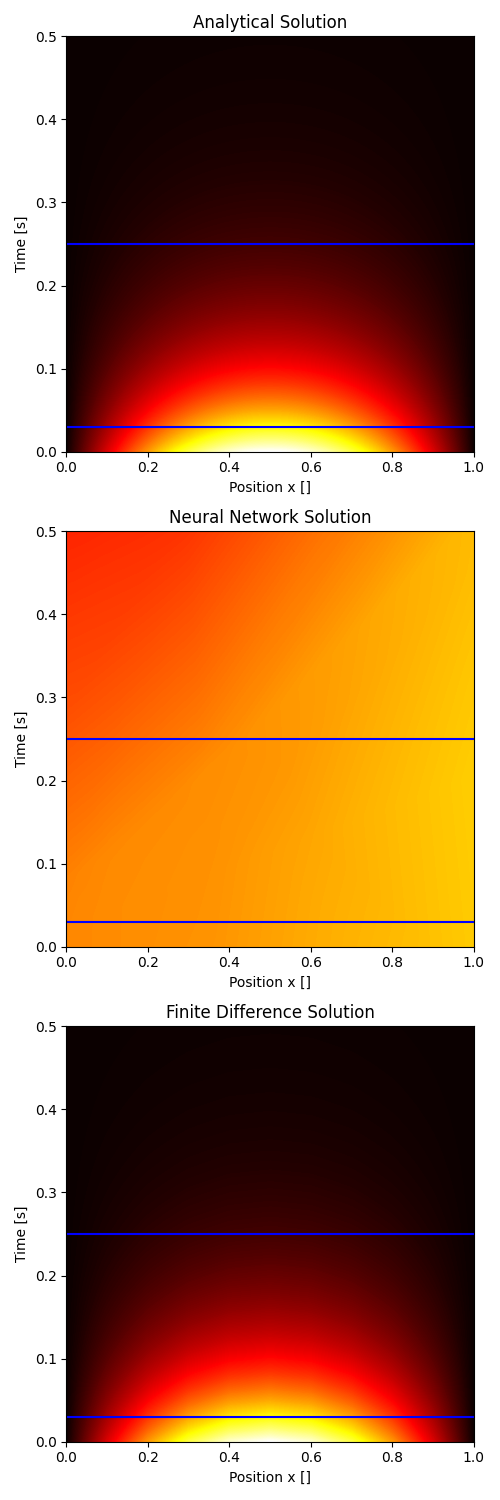
\includegraphics[width=1.0\linewidth]{project_3/plots/heat_map_comparison.png}
    \caption{The analytical solution to the heat equation, and the results from the finite difference method and the neural network model. A common color bar is displayed as all three plots have the same range of values [0,1]. The color bar is showing the $Temperature$. The blue lines indicate the times $t_1 = 0.03 s$ and $t_2 = 0.40 s$.}
    \label{fig:heatmaps}
\end{figure}

The results from the finite difference method and the neural network are presented in Fig. \ref{fig:heatmaps}.
In this plot, the outputs from the finite difference model have been interpolated making it appear smooth even though the model only outputs a discrete set of values. 
There is no noticeable difference by eye between the three plots, which is well reflected in the very low MSE-value observed in both numerical methods. 
Compared to the analytical solution, the output of the neural network model has an MSE of $ 6.71 \times 10^{-6}$ while the finite difference method yields an MSE of $2.52 \times 10^{-7}$. 

Since we considered different discretizations of the grid for the two methods, the analytical solution is evaluated only at the respective grid points of each method. 
Consequently, the MSE calculation for the neural network involves a greater number of points than that of the finite difference method.
As the finite difference model only provides predictions for a predefined set of discrete points, it does not make sense to calculate its MSE on a set of points with finer granularity.
However, the resolution of points used to calculate the MSE will not have a substantial impact on its value, hence the MSE values are still comparable.

\begin{figure}[h!]
    \centering
    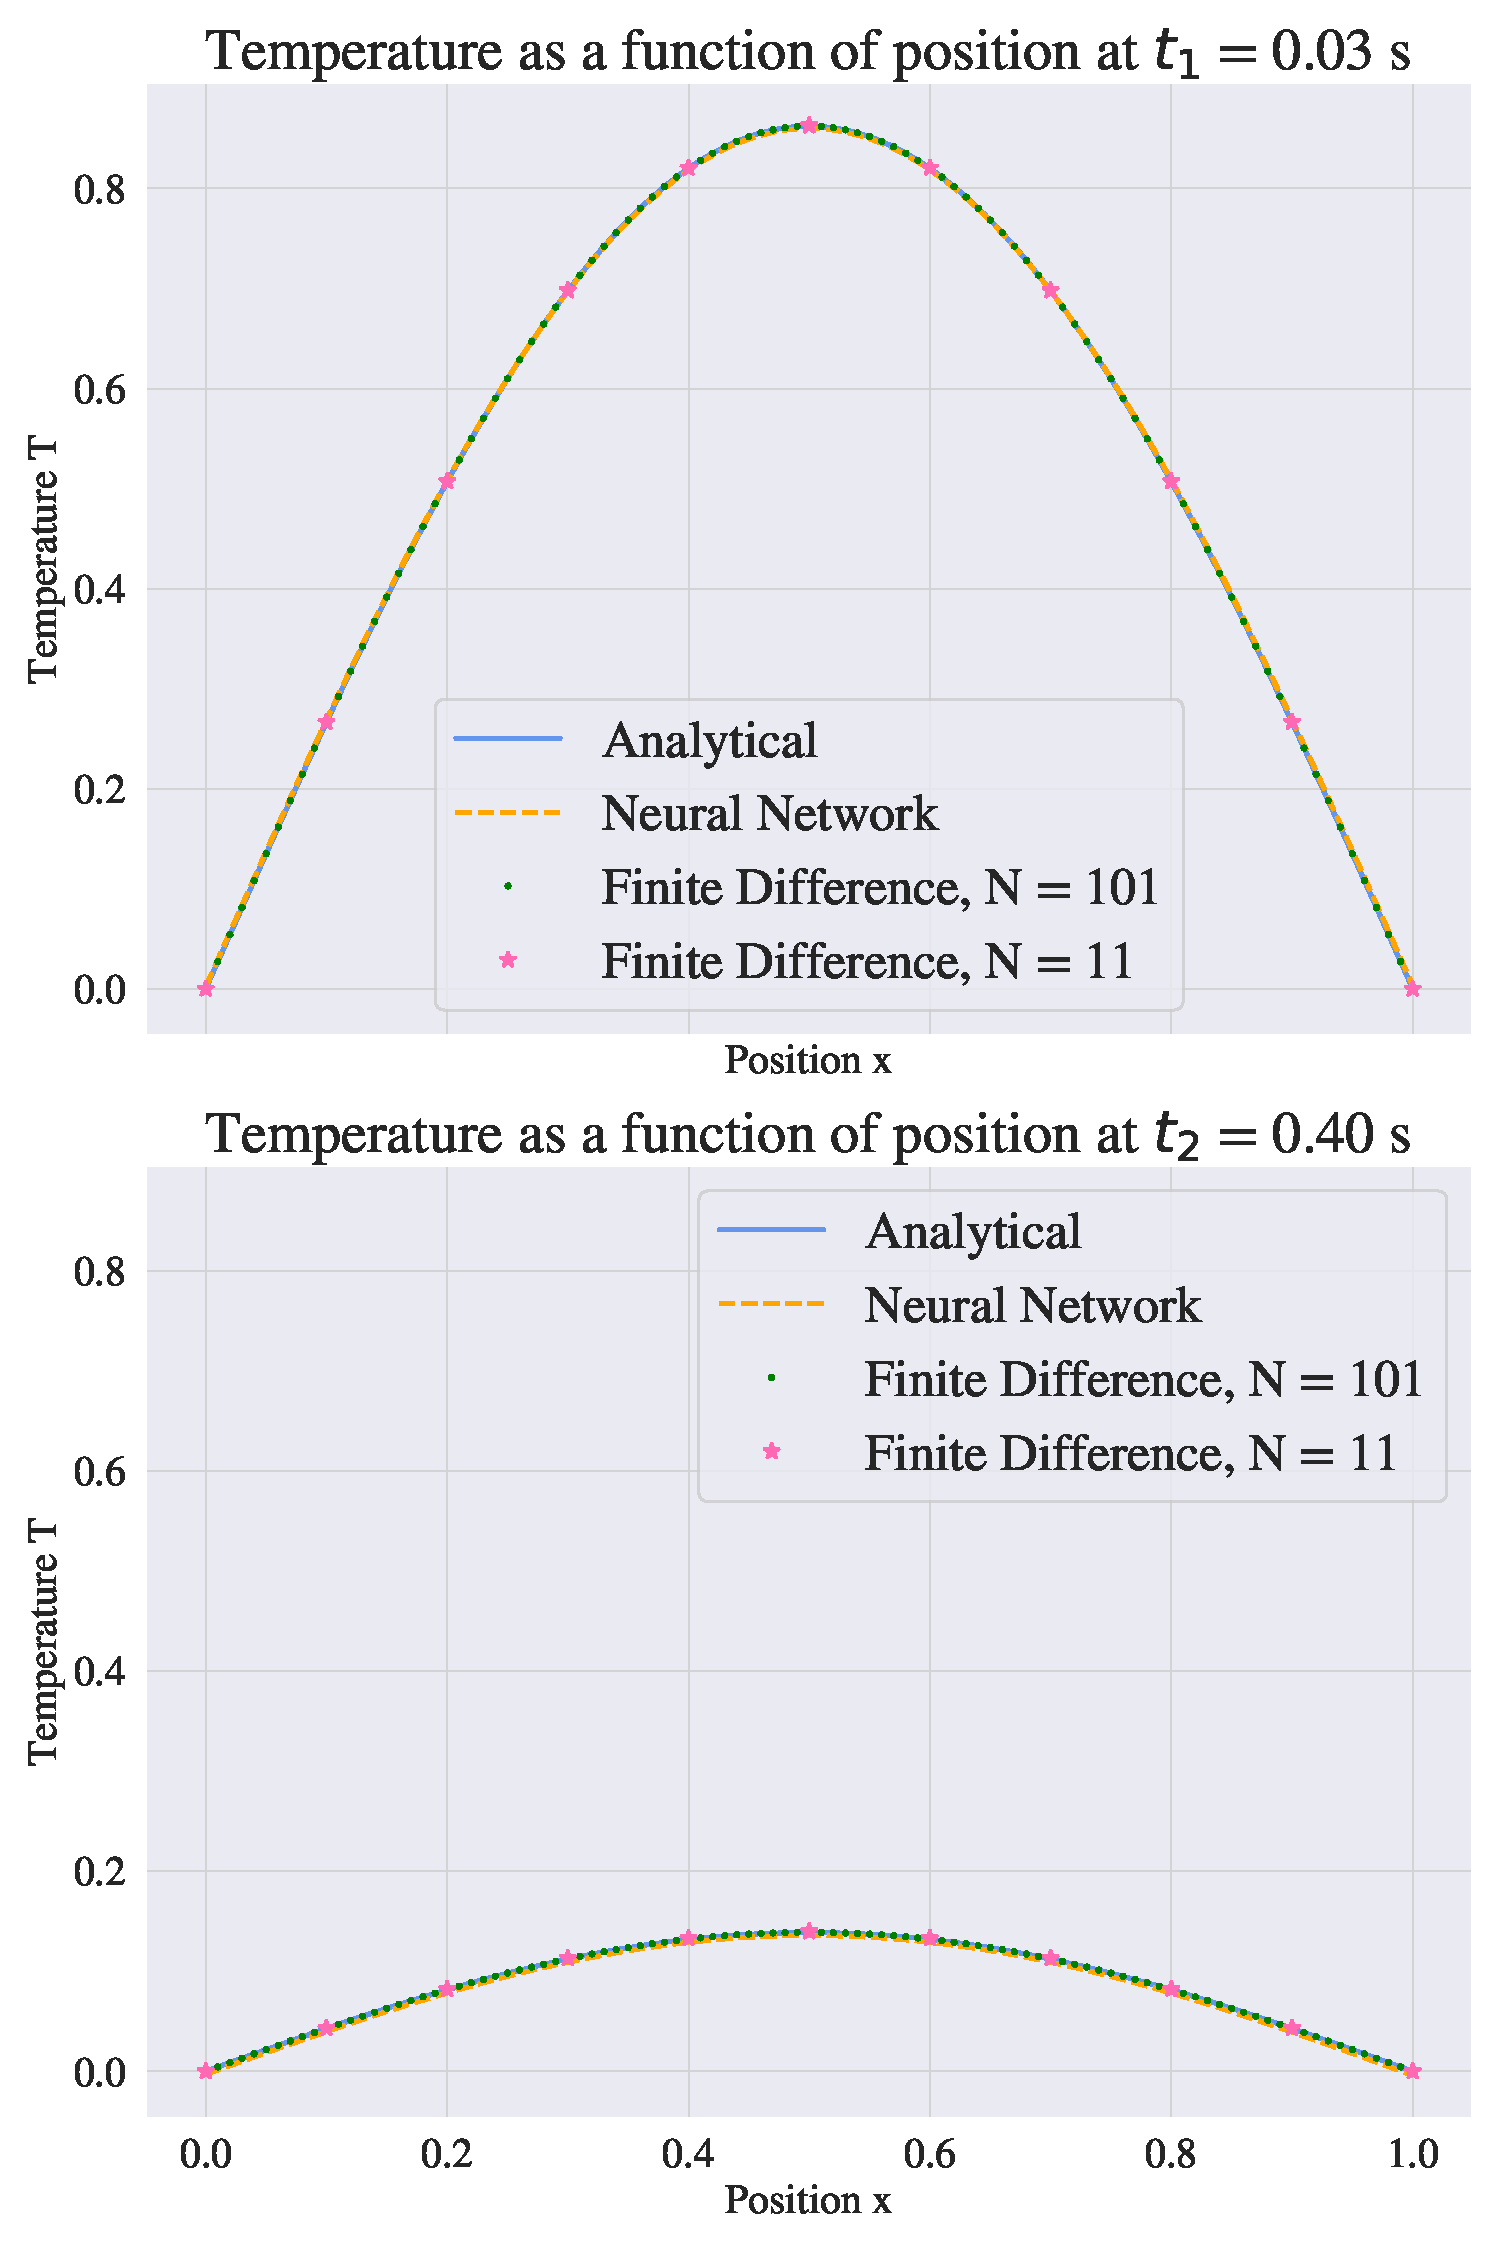
\includegraphics[width=1.0\linewidth]{project_3/plots/time_slices_comparison.pdf}
    \caption{The temperature for specific times for the analytical solution, as well as the output from the finite difference method and the neural network predictions. The discretization along the x-axis is different for each method. The analytical one is plotted with 1000 points, the finite difference method with 11 and 101 points, and the neural network predictions with 100. }
    \label{fig:timeslices}
\end{figure}


We ``\textit{slice}" the heatmaps in Fig. \ref{fig:heatmaps} at two specific times, $t_1 = 0.03 s$ and $t_2 = 0.40 s$. 
This is illustrated as blue lines in Fig. \ref{fig:heatmaps}.
The temperature values across the x-range are plotted for all three cases in Fig. \ref{fig:timeslices}.
At $t_1$, the function is still significantly curved, while at $t_2$ it has almost reached the stationary state.
This serves as an additional verification of the previously presented results. 
The finite difference methods seems to match the analytical solution to a high accuracy in its discrete points, while the neural network ever so slightly undershoots it.
The effect of this is more prominent for the later time stamp $t_2$. 
These results reflect the difference in MSE between the finite difference method and the neural network, with the former performing slightly better. 

% In comparison of the two we also consider that the finite difference method is designed specifically for approximating partial differential equations, while neural networks can approximate more or less any function.
In comparison of the two we take into consideration that the construction of the finite difference scheme relies on deeper mathematical knowledge about partial derivatives, such as Taylor series.
Opposingly, the neural network only has the exact equation with initial and boundary conditions, which in practice means it has less information than the finite difference method.
Additionally, the finite difference scheme is designed to approximate a finite selection of discrete points, while the neural network attempts a continuous approximation for the entire function. This might favor the finite difference model in the comparison, as it has no constraints for a smooth prediction across the domain. 

It should be noted that we are not feeding the neural network any actual data points, only the pure PDE problem through the cost function.
In practical application of PDEs, one would combine data with a tailor-made cost-function in order to obtain the best physics-informed neural network possible.
That said, the finite difference scheme does neither receive any other data than the PDE itself combined with its initial conditions and boundary values, hence we conclude that this does not skew the comparison.

The finite difference method requires a larger process of programming based on the specific PDE problem it is made to solve.
That said, after the problem is implemented, there is no need for further tuning of any hyperparameters.
The method is however limited to only solving PDE problems based on known PDEs, initial conditions and boundary values.

Physics-informed neural networks on the other hand, offers a more flexible type of model where one neural network can solve a number of PDE problems only by changing the cost function.
They can also combine other types of problem structures, such as a PDE with unknown coefficients, or missing initial or boundary values, by combining that information with sampled points form the solution (e.g. some measured values in physical experiments).
This makes them more versatile for different real life application.

Still, they do have some major disadvantages: They require far more computational power than most finite difference models, as well as needing a lot of hyperparameter tuning.
Furthermore, the fact that they output a continuous function is not a big advantage, as this function is complex and hard to interpret.
In the case that one seeks a continuous result, the function one obtains from interpolating the values of a finite difference method might be just as good, given a fine enough granularity. 
